\begin{enumerate}[label=\bfseries Câu \arabic*:]
	
	
	%%%%%%%%%%%%%%CÂU2%%%%%%%%%%
	\item \mkstar{1}
	
	\cauhoi{Phát biểu nào sau đây là \textbf{không} đúng?
		\begin{mcq}(1)
			\item Công suất của dòng điện xoay chiều phụ thuộc vào công suất hao phí trên đường dây tải điện.
			\item Công suất của dòng điện xoay chiều phụ thuộc vào hiệu điện thế hiệu dụng giữa hai đầu đoạn mạch.
			\item Công suất của dòng điện xoay chiều phụ thuộc vào cường độ dòng điện hiệu dụng trong mạch.
			\item Công suất của dòng điện xoay chiều phụ thuộc vào bản chất của mạch điện và tần số dòng điện trong mạch.
		\end{mcq}
	}	
	\loigiai{
		\textbf{Đáp án: A.}
		
		Công suất của dòng điện xoay chiều được tính theo công thức $P=UI\cos\varphi$. Suy ra công suất của dòng điện xoay chiều phụ thuộc vào cường độ dòng điện hiệu dụng I trong mạch, điện áp hiệu dụng U giữa hai đầu đoạn mạch, bản chất của mạch điện và tần số dòng điện trong mạch (đặc trưng bởi độ lệch pha).
		
	}
	
	%%%%%%%%%%%%%%CÂU3%%%%%%%%%%

	
	%%%%%%%%%%%%%%CÂU4%%%%%%%%%%
	\item \mkstar{1}
	
	\cauhoi{Công suất của dòng điện xoay chiều trên đoạn mạch RLC nối tiếp \textbf{không} phụ thuộc vào đại lượng nào sau đây?
		\begin{mcq}
			\item Hiệu điện thế cực đại giữa hai đầu đoạn mạch.
			\item Cường độ hiệu đụng của dòng điện qua mạch.
			\item Độ lệch pha giữa dòng điện và hiệu điện thế giữa hai bản tụ.
			\item Tỉ số giữa điện trở thuần và tổng trở của mạch.
		\end{mcq}
	}	
	\loigiai{
		\textbf{Đáp án: C.}
		
		Độ lệch pha giữa dòng điện và điện áp giữa hai đầu tụ điện luôn là $\dfrac{\pi}{2}$.
		
	}
	
	%%%%%%%%%%%%%%CÂU5%%%%%%%%%%

	
	%%%%%%%%%%%%%%CÂU7%%%%%%%%%%
	\item \mkstar{1}
	
	\cauhoi{Trong các dụng cụ tiêu thụ điện như quạt, tủ lạnh, động cơ, người ta năng cao hệ số công suất nhằm
		\begin{mcq}(2)
			\item tăng cường độ dòng điện.
			\item tăng công suất tiêu thụ.
			\item giảm cường độ dòng điện.
			\item giảm công suất tiêu thụ.
		\end{mcq}
	}	
	\loigiai{
		\textbf{Đáp án: C.}
		
		Trong các dụng cụ tiêu thụ điện như quạt, tủ lạnh, động cơ, người ta năng cao hệ số công suất nhằm giảm cường độ dòng điện, giảm hao phí tỏa nhiệt và nâng cao hiệu suất.
		
	}
	
	%%%%%%%%%%%%%%CÂU8%%%%%%%%%%
	
	%%%%%%%%%%%%%%CÂU9%%%%%%%%%%
\item \mkstar{2}

\cauhoi{Công suất của dòng điện xoay chiều trên một đoạn mạch $RLC$ nối tiếp nhỏ hơn tích $UI$ là do
	\begin{mcq}
		\item một phần điện năng tiêu thụ trong tụ điện.
		\item trong cuộn dây có dòng điện cảm ứng.
		\item điện áp giữa hai đầu đoạn mạch và cường độ dòng điện lệch pha không đổi với nhau.
		\item có hiện tượng cộng hưởng điện trên đoạn mạch.
	\end{mcq}
}
	\loigiai{
		\textbf{Đáp án: C.}
		
		Công suất của dòng điện xoay chiều trên một đoạn mạch $RLC$ nối tiếp nhỏ hơn tích $UI$ là do điện áp giữa hai đầu đoạn mạch và cường độ dòng điện lệch pha không đổi với nhau.
		
		}


%%%%%%%%%%%%%%CÂU3%%%%%%%%%%
\item \mkstar{2}

\cauhoi{Một điện áp xoay chiều được đặt vào hai đầu một điện trở thuần. Giữ nguyên giá trị hiệu dụng, thay đổi tần số của điện áp. Công suất toả nhiệt trên điện trở
	\begin{mcq}
		\item tỉ lệ thuận với bình phương của tần số.
		\item tỉ lệ thuận với tần số.
		\item tỉ lệ nghịch với tần số.
		\item không phụ thuộc vào tần số.
	\end{mcq}
}	
	\loigiai{
		\textbf{Đáp án: D.}
		
		$\calP=UI\cos\varphi=I^2R$.
		
		}


%%%%%%%%%%%%%%CÂU4%%%%%%%%%%
\item \mkstar{2}

\cauhoi{Đoạn mạch điện nào sau đây có hệ số công suất lớn nhất?
	\begin{mcq}
		\item Điện trở thuần $R_1$ nối tiếp với điện trở thuần $R_2$.
		\item Điện trở thuần $R$ nối tiếp với cuộn cảm $L$.
		\item Điện trở thuần $R$ nối tiếp với tụ điện $C$.   
		\item Cuộn cảm $L$ nối tiếp với tụ điện $C$.
	\end{mcq}
}	
	\loigiai{
		\textbf{Đáp án: A.}
		
		$\cos\varphi=\dfrac{R}{Z}$.
		
		}




%%%%%%%%%%%%%%CÂU5%%%%%%%%%%
\item \mkstar{2}

\cauhoi{Công suất tức thời của dòng điện xoay chiều
	\begin{mcq}
		\item luôn biến thiên với tần số bằng hai lần tần số của dòng điện.
		\item có giá trị trung bình biến thiên theo thời gian.
		\item không thay đổi theo thời gian, tính bằng công thức $\calP=UI\cos\varphi$.
		\item luôn biến thiên cùng pha, cùng tần số với dòng điện.
	\end{mcq}
}	
	\loigiai{
		\textbf{Đáp án: A.}
		
		Công suất tức thời của dòng điện xoay chiều luôn biến thiên với tần số bằng hai lần tần số của dòng điện.
		
		}


%%%%%%%%%%%%%%CÂU6%%%%%%%%%%
\item \mkstar{2}

\cauhoi{Trong mạch điện xoay chiều không phân nhánh, điện áp giữa hai đầu đoạn mạch và cường độ dòng điện trong mạch lần lượt là $u=100\cos 100\pi t\,\text{V}$ và $i=100\cos\left(100\pi t+\dfrac{\pi}{3}\right)\,\text{mA}$. Công suất tiêu thụ trong mạch là
	\begin{mcq}(4)
		\item $\SI{5000}{\watt}$.
		\item $\SI{2500}{\watt}$.
		\item $\SI{50}{\watt}$.
		\item $\SI{2,5}{\watt}$.
	\end{mcq}
}	
	\loigiai{
		\textbf{Đáp án: D.}
		
		$\calP=UI\cos\varphi=\SI{2,5}{\watt}.$
		
		}


%%%%%%%%%%%%%%CÂU7%%%%%%%%%%
\item \mkstar{2}

\cauhoi{Đặt một điện áp xoay chiều $\SI{100}{V}-\SI{50}{Hz}$ vào hai đầu một cuộn dây có điện trở là $r=\SI{10}{\ohm}$ thì dòng điện chạy qua cuộn dây lệch pha $\dfrac{\pi}{3}$ so với điện áp đó. Công suất tiêu thụ của cuộn dây là
	\begin{mcq}(4)
		\item $\SI{600}{\watt}$.
		\item $\SI{500}{\watt}$.
		\item $\SI{250}{\watt}$.
		\item $\SI{125}{\watt}$.
	\end{mcq}
}	
	\loigiai{
		\textbf{Đáp án: C.}
		
		$\calP=I^2R=UI\cos\varphi=\dfrac{U^2}{R}\cos^2\varphi=\SI{250}{\watt}$.
		
		}


%%%%%%%%%%%%%%CÂU8%%%%%%%%%%


%%%%%%%%%%%%%%CÂU10%%%%%%%%%%

	%%%%%%%%%%%%%%CÂU13%%%%%%%%%%
	\item \mkstar{2}
	
	\cauhoi{Đặt vào hai đầu đoạn mạch $RLC$ mắc nối tiếp một hiệu điện thế dao động điều hòa có biểu thức $u=220\sqrt{2}\cos\omega t\,\text{V}$. Biết điện trở thuần của mạch có giá trị là $\SI{100}{\ohm}$. Khi $\omega$ thay đổi thì công suất tiêu thụ cực đại của mạch có giá trị là
		\begin{mcq}(4)
			\item $\SI{440}{\watt}$.
			\item $\SI{484}{\watt}$.
			\item $\SI{220}{\watt}$.
			\item $\SI{242}{\watt}$.
		\end{mcq}
	}	
	\loigiai{
		\textbf{Đáp án: B.}
		
		Khi $\omega$ thay đổi để $P_\text{max}$ thì hiện tượng cộng hưởng xảy ra
		$$P_\text{max}=\dfrac{U^2}{R}=\SI{484}{\watt}.$$
		
	}
\item \mkstar{2}

\cauhoi{Đặt một điện áp xoay chiều vào hai đầu đoạn mạch $RLC$ nối tiếp có $R$ thay đổi thì thấy khi $R=\SI{30}{\ohm}$ và $R=\SI{120}{\ohm}$ thì công suất tỏa nhiệt trên đoạn mạch không đổi. Để công suất đó đạt cực đại thì giá trị $R$ phải là
	\begin{mcq}(4)
		\item $\SI{150}{\ohm}$.
		\item $\SI{24}{\ohm}$.
		\item $\SI{90}{\ohm}$.
		\item $\SI{60}{\ohm}$.
	\end{mcq}
}	
\loigiai{
	\textbf{Đáp án: D.}
	
	$R\sqrt{R_1R_2}=\SI{60}{\ohm}.$
	
}


%%%%%%%%%%%%%%CÂU9%%%%%%%%%%
\item \mkstar{2}

\cauhoi{Một đoạn mạch nối tiếp gồm một cuộn dây và một tụ điện. Hiệu điện thế hiệu dụng giữa hai đầu đoạn mạch, giữa hai đầu cuộn dây, hai đầu tụ điện đều bằng nhau. Tìm hệ số công suất $\cos\varphi$ của mạch.
	\begin{mcq}(4)
		\item 0,5.
		\item $\dfrac{\sqrt{3}}{2}$.
		\item $\dfrac{\sqrt{2}}{2}$.
		\item $\dfrac{1}{4}$.
	\end{mcq}
}	
\loigiai{
	\textbf{Đáp án: B.}
	
	Ta đặt $U=U_\text{d}=U_C=1$.
	
	Ta có $U^2=U_r^2+(U_L-U_C)^2\Rightarrow 1=U_r^2+(U_L-1)^2$.
	
	và $U_\text{d}^2=U_r^2+U_L^2\Rightarrow 1=U_r^2+U_L^2$.
	
	Từ đó ta suy ra $U_L=0,5$, $U_r=\dfrac{\sqrt{3}}{2}$.
	
	Hệ số công suất $\cos\varphi$ của mạch là $\cos\varphi=\dfrac{U_r}{U}=\dfrac{\sqrt{3}}{2}$.
	
}

	%%%%%%%%%%%%%%CÂU15%%%%%%%%%%
	\item \mkstar{3}
	
	\cauhoi{Cho đoạn mạch không phân nhánh $RLC$, $R=\SI{80}{\ohm}$,cuộn dây có điện trở trong $\SI{20}{\ohm}$ và độ tự cảm $L=\SI{0,318}{H}$, tụ điện có điện dung $\SI{15,9}{\micro\farad}$. Đặt vào hai đầu mạch điện một dòng điện xoay chiều có tần số $f$ thay đổi được có hiệu điện thế hiệu dụng là $\SI{200}{V}$.Khi công suất trên toàn mạch đạt giá trị cực đại thì giá trị của $f$ và $\calP$ bằng bao nhiêu?
		\begin{mcq}(2)
			\item $\SI{70,78}{Hz}$ và $\SI{400}{\watt}$.
			\item $\SI{70,78}{Hz}$ và $\SI{500}{\watt}$.
			\item $\SI{444,7}{Hz}$ và $\SI{2000}{\watt}$.
			\item $\SI{31,48}{Hz}$ và $\SI{400}{\watt}$.
		\end{mcq}
	}	
	\loigiai{
		\textbf{Đáp án: A.}
		
		Khi cường độ dòng điện trong mạch cực đại thì cộng hưởng điện xảy ra. Khi đó cường độ dòng điện cực đại là
		$$I=\dfrac{U}{R+r}=\SI{2}{A}.$$
		
		Tần số dòng điện là
		$$f=\dfrac{\omega}{2\pi}=\dfrac{1}{2\pi\sqrt{LC}}=\SI{70,78}{Hz}.$$
		
		Công suất cực đại là $P=I^2(R+r)=\SI{400}{\watt}$.
		
	}
	
	%%%%%%%%%%%%%%CÂU16%%%%%%%%%%
	\item \mkstar{3}
	
	\cauhoi{Đặt vào hai đầu đoạn mạch $RLC$ mắc nối tiếp một hiệu điện thế dao động điều hòa có biểu thức $u=220\cos\omega t\, \text{V}$. Khi $\omega$ thay đổi công suất tiêu thụ cực đại của mạch là $\SI{484}{\watt}$. Khi đó điện trở thuần của mạch là
		\begin{mcq}(4)
			\item $R=\SI{50}{\ohm}$.
			\item $R=\SI{750}{\ohm}$.
			\item $R=\SI{150}{\ohm}$.
			\item $R=\SI{100}{\ohm}$.
		\end{mcq}
	}	
	\loigiai{
		\textbf{Đáp án: A.}
		
		Khi $\omega$ thay đổi để công suất cực đại thì có cộng hưởng. Điện trở thuần của mạch là
		$$R=\dfrac{U^2}{P}=\SI{50}{\ohm}.$$
		
	}
\item \mkstar{3}

\cauhoi{Một đoạn mạch xoay chiều gồm cuộn dây có điện trở $R$, độ tự cảm $L$ nối tiếp với một tụ điện có điện dung $C$ đặt dưới điện áp xoay chiều có giá trị hiệu dụng ổn định. Cường độ dòng điện qua mạch là $i_1=3\cos100\pi t\,\text{A}$. Nếu tụ điện bị nối tắt thì cường độ dòng điện qua mạch là $i_2=3\cos\left(100\pi t+\dfrac{\pi}{3}\right)\,\text{A}$. Hệ số công suất trong hai trường hợp trên lần lượt là
	\begin{mcq}(2)
		\item $\cos\varphi_1=1$, $\cos\varphi_2=\dfrac{1}{2}$.
		\item $\cos\varphi_1=\cos\varphi_2=\dfrac{\sqrt{3}}{2}$.
		\item $\cos\varphi_1=\cos\varphi_2=\dfrac{3}{4}$.
		\item $\cos\varphi_1=\cos\varphi_2=\dfrac{1}{2}$.
	\end{mcq}
}	
\loigiai{
	\textbf{Đáp án: B.}
	
	Lúc đầu mạch là $RLC$ thì dòng điện $i_1=3\cos100\pi t\,\text{A}$.
	
	Khi nối tắt tụ điện thì mạch chỉ còn $RL$ cường độ dòng điện là $i_2=3\cos\left(100\pi t+\dfrac{\pi}{3}\right)\,\text{A}$.
	
	Ta thấy $I_{01}=I_{02}=\SI{3}{A}$. Do đó $Z_{RLC}=Z_{RL}$. Từ đó suy ra $\cos\varphi_1=\cos\varphi_2=\dfrac{\sqrt{3}}{2}$.	
	
}	
	%%%%%%%%%%%%%%CÂU17%%%%%%%%%%
	\item \mkstar{3}
	
	\cauhoi{Đoạn mạch xoay chiều gồm điện trở $R$, tụ điện có điện dung $C$ thay đổi được, cuộn dây có độ tự cảm $L=\dfrac{1}{\pi}\,\text{H}$ và điện trở $r=\SI{20}{\ohm}$ mắc nối tiếp. Đặt vào hai đầu đoạn mạch điện áp xoay chiều có giá trị hiệu dụng $U=\SI{60}{V}$ và tần số $f=\SI{50}{Hz}$. Điều chỉnh điện dung tụ điện đến giá trị $C_1$ thì công suất tiêu thụ trên mạch đạt cực đại và bằng $\SI{30}{\watt}$. Điện trở $R$ và điện dung $C_1$ có giá trị là
		\begin{mcq}(2)
			\item $R=\SI{120}{\ohm}$; $C_1=\dfrac{10^4}{2\pi}\,\text{F}$.
			\item $R=\SI{120}{\ohm}$; $C_1=\dfrac{10^4}{\pi}\,\text{F}$.
			\item $R=\SI{100}{\ohm}$; $C_1=\dfrac{10^4}{2\pi}\,\text{F}$.
			\item $R=\SI{100}{\ohm}$; $C_1=\dfrac{10^4}{\pi}\,\text{F}$.
		\end{mcq}
	}	
	\loigiai{
		\textbf{Đáp án: D.}
		
		Khi $C$ thay đổi để công suất cực đại thì xảy ra hiện tượng cộng hưởng nên $C=\dfrac{10^4}{\pi}\,\text{F}$.
		
		Điện trở là $R=\dfrac{U^2}{P_\text{max}}-r=\SI{100}{\ohm}$.
		
	}

	\item \mkstar{3}
	
	\cauhoi{Cho mạch điện gồm $R$, $L$, $C$ mắc nối tiếp. Biết $R=\SI{30}{\ohm}$, $R=\SI{0,4}{H}$, $C$ thay đổi được. Đặt vào hai đầu mạch điện một hiệu điện thế xoay chiều $u=120\cos(100t+\pi/2)\,\text{V}$. Khi $C=C_0$ thì công suất trong mạch đạt giá trị cực đại. Khi đó biểu thức điện áp giữa hai đầu điện trở là
		\begin{mcq}(2)
			\item $u_R=60\sqrt{2}\cos100t\,\text{V}$.
			\item $u_R=120\sqrt{2}\cos(100t+\pi/2)\,\text{V}$.
			\item $u_R=120\sqrt{2}\cos100t\,\text{V}$.
			\item $u_R=60\sqrt{2}\cos(100t+\pi/2)\,\text{V}$.
		\end{mcq}
	}	
	\loigiai{
		\textbf{Đáp án: B.}
		
		Ta có cảm kháng là $Z_L=\omega L=\SI{40}{\omega}$.
		
		Khi $C$ thay đổi để công suất tiêu thụ cực đại thì $Z_L=Z_C=\SI{40}{\ohm}$.
		
		Do đó $u_R$ cùng pha với $u$ nên $u_R=120\sqrt{2}\cos(100t+\pi/2)\,\text{V}$.
		
	}
	
	%%%%%%%%%%%%%%CÂU19%%%%%%%%%%

	%%%%%%%%%%%%%%CÂU3%%%%%%%%%%
	\item \mkstar{4}
	
	\cauhoi{Đặt điện áp $u=U_0\cos \omega t$  ($U_0$, $\omega$  không đổi) vào đoạn mạch mắc nối tiếp gồm điện trở $R$, tụ điện có điện dung $C$ và cuộn cảm thuần có độ tự cảm $L$ thay đổi. Hình vẽ bên là đồ thị biểu diễn sự phụ thuộc của điện áp hiệu dụng $U_L$ giữa hai đầu cuộn cảm và hệ số công suất $\cos \varphi$  của đoạn mạch theo giá trị của độ tự cảm $L$. Giá trị của $U_0$ gần nhất với giá trị nào sau đây?
		\begin{center}
			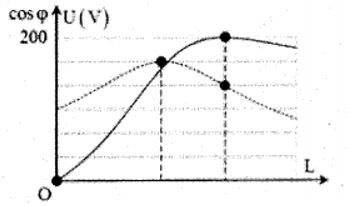
\includegraphics[scale=0.9]{../figs/VN12-PH-19-P-013-1-2.jpg}
		\end{center}
		\begin{mcq}(4)
			\item 240 V.
			\item 165 V.
			\item 220 V.
			\item 185 V.
		\end{mcq}
	}
	\loigiai{
		\textbf{Đáp án: B.}
		
		Khi xảy ra cực đại của điện áp hiệu dụng trên cuộn cảm thuần $$Z_L = \dfrac{R^2+Z^2_C}{Z_C}$$.
		
		Ta chuẩn hóa $R=1; Z_C = n \Rightarrow Z_L =\dfrac{1}{x} +x$.
		
		Hệ số công suất của mạch tương ứng $$\cos \varphi =\dfrac{R}{\sqrt{R^2 + (Z_L - Z_C)^2}} \Leftrightarrow \text{0,8} =\dfrac{1}{\sqrt {1+ \dfrac{1}{n^2}}} \Rightarrow n =\dfrac{4}{3}$$.
		
		Kết hợp với $$U_{L\text{max}} = U\sqrt {1+ \left (\dfrac{Z_C}{R}\right)^2} \Rightarrow U = \dfrac{U_{L_\text{max}}}{\sqrt {1+\left (\dfrac{Z_C}{R}\right)^2 }} =120\ \text{V}$$
		
		Suy ra $U_0 =120\sqrt 2 \approx 170\ \text{V}$.
		
		
	}
	
	%%%%%%%%%%%%%%CÂU4%%%%%%%%%%
	

	%%%%%%%%%%%%%%CÂU6%%%%%%%%%%
	\item \mkstar{4}
	
	\cauhoi{Đặt một điện áp xoay chiều có giá trị hiệu dụng và tần số không đổi vào hai đầu đoạn mạch điện AB gồm biến trở $R$, tụ điện $C$ và cuộn dây không thuần cảm có độ tự cảm $L$, điện trở thuần $r$, ghép nối tiếp với nhau như hình vẽ.
		\begin{center}
			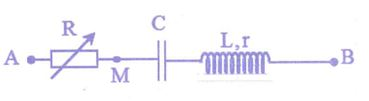
\includegraphics[scale=1]{../figs/VN12-PH-19-P-013-1-5.jpg}
		\end{center}
		Điều chỉnh R đến giá trị $60\ \Omega$ thì công suất tiêu thụ trên biến trở đạt cực đại, đồng thời tổng trở của đoạn mạch AB là số nguyên chia hết cho 45. Khi đó hệ số công suất của đoạn mạch MB có giá trị là
		
		\begin{mcq}(4)
			\item 0,375.
			\item 0,75.
			\item 0,125.
			\item 0,5.
		\end{mcq}
	}	
	\loigiai{
		\textbf{Đáp án: C.}
		
		Giá trị của biến trở để công suất tiêu thụ trên biến trở là cực đại:
		
		$$R=R_0 = \sqrt{r^2 +(Z_L-Z_C)^2} = 60\ \Omega$$
		
		+ Tổng trở của mạch khi đó
		
		$$Z= \sqrt{(R_0 +r)^2 +(Z_L-Z_C)^2} = \sqrt {R_0^2 + 2R_0r +r^2 +(Z_L-Z_C)^2}$$
		$$\Rightarrow Z^2 = 60^2 +2 \cdot 60 r + 60^2 = (n \cdot 45)^2 \Rightarrow r =\dfrac{135}{8}n^2 -60$$
		
		+ Hệ số công suất của đoạn mạch MB:
		
		$$\cos \varphi_\text{MB} = \dfrac{r}{\sqrt {r^2 + (Z_L-Z_C)^2 }} = \dfrac{\dfrac{135}{8}n^2 -60}{60}$$
		$$ 0<\cos \varphi_\text{MB} <1 \Leftrightarrow \text{1,89}<n<\text{2,7}$$
		
		$n=2$ suy ra $\cos \varphi_\text{MB} =\text{0,125}$. 
		
	}
	
	%%%%%%%%%%%%%%CÂU7%%%%%%%%%%
	
	
	%%%%%%%%%%%%%%CÂU8%%%%%%%%%%
	\item \mkstar{4}
	
	\cauhoi{Cho mạch điện như hình vẽ, cuộn dây thuần cảm. Điện áp hai đầu đoạn mạch có biểu thức $u= U\sqrt 2\cos 2\pi f t\ \text{V}$  với $U$ không đổi nhưng $f$ có thể thay đổi được. Ta có đồ thị biểu diễn sự phụ thuộc của công suất tiêu thụ trên mạch theo $R$ là đường liền nét khi $f=f_1$  và là đường đứt nét khi $f=f_2$. Giá trị của $P_\text{max}$  gần nhất với giá trị nào sau đây?
		\begin{center}
			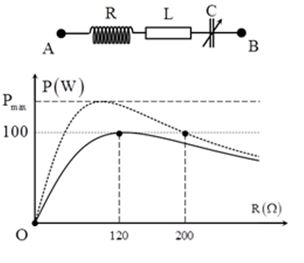
\includegraphics[scale=1.1]{../figs/VN12-PH-19-P-013-1-7.jpg}
		\end{center}
		\begin{mcq}(4)
			\item 280 W.
			\item 140 W.
			\item 130 W.
			\item 260 W.
		\end{mcq}
	}		
	\loigiai{
		\textbf{Đáp án: C.}
		
		+	$f=f_1$: Công suất cực đại của mạch khi $R_0 =120 = |Z_{L_1} - Z_{C_1}|.$
		
		Khi đó: $$P_{\text{max}_1} = \dfrac{U^2}{2|Z_{L_1} - Z_{C_1}|} \Rightarrow 100 =\dfrac{U^2}{2 \cdot 120} \Rightarrow U = 40\sqrt {15} \ \text{V}$$
		
		+ $f=f_2$: khi $R=200\ \Omega$ thì công suất tiêu thụ của mạch là 100 W.
		
		$$\Rightarrow 100 = \dfrac{(40\sqrt{15})^2}{200^2 + (Z_{L_2}-Z_{C_2})^2} \cdot 200 \Rightarrow |Z_{L_2}-Z_{C_2}| =40\sqrt 5.$$
		
		Khi đó: $P_\text{max} = P_{\text{max}_2} = \dfrac{U^2}{2|Z_{L_2}-Z_{C_2}|} =60\sqrt 5 \approx \text{134,16}\ \text{W}$.
		
		
	}
	
	%%%%%%%%%%%%%%CÂU9%%%%%%%%%%

\end{enumerate}
\loigiai{\textbf{Đáp án}
	\begin{center}
		\begin{tabular}{|m{2.8em}|m{2.8em}|m{2.8em}|m{2.8em}|m{2.8em}|m{2.8em}|m{2.8em}|m{2.8em}|m{2.8em}|m{2.8em}|}
			\hline
			1. A & 2. C & 3. C & 4. C & 5. D & 6. A  & 7. A  & 8. D & 9. C & 10. B\\
			\hline
			11. D & 12. B & 13. A & 14. A & 15. B & 16. D  & 17. B  & 18. B & 19. C & 20. C\\
			\hline
		\end{tabular}
\end{center}}